\documentclass[9pt,aspectratio=169,xcolor=table]{beamer}

%~~~~~~~~~~~~~~~~~~~~~~~~~~~~~~~~~~~~~~~~~~~~~~~~~~~~~~~~~~~~~~~~~~~~~~~~~~~~~~
% Use roboto Font (recommended)
\usepackage[sfdefault]{roboto}
\usepackage[utf8]{inputenc}
\usepackage[T1]{fontenc}
%~~~~~~~~~~~~~~~~~~~~~~~~~~~~~~~~~~~~~~~~~~~~~~~~~~~~~~~~~~~~~~~~~~~~~~~~~~~~~~

%~~~~~~~~~~~~~~~~~~~~~~~~~~~~~~~~~~~~~~~~~~~~~~~~~~~~~~~~~~~~~~~~~~~~~~~~~~~~~~
% Define where theme files are located. ('/styles')
\usepackage{styles/fluxmacros}
\usefolder{styles}
% Use Flux theme v0.1 beta
% Available style: asphalt, blue, red, green, gray
% "red" is the closest built-in style to maroon; its exact colours are
% overridden with a true maroon palette just below, after the theme loads.
\usetheme[style=red]{flux}
%~~~~~~~~~~~~~~~~~~~~~~~~~~~~~~~~~~~~~~~~~~~~~~~~~~~~~~~~~~~~~~~~~~~~~~~~~~~~~~

%~~~~~~~~~~~~~~~~~~~~~~~~~~~~~~~~~~~~~~~~~~~~~~~~~~~~~~~~~~~~~~~~~~~~~~~~~~~~~~
% SKEE1033 maroon palette override.
\definecolor{primaryLight}{HTML}{9B2242} % lighter maroon -- headers, accents
\definecolor{primary}{HTML}{7B1E3A}      % core maroon -- titles, block headers
\definecolor{secondary}{HTML}{3A5A6B}    % muted teal -- complementary accent
\definecolor{tertiary}{HTML}{8C6A3F}     % warm bronze -- example/third accent
%~~~~~~~~~~~~~~~~~~~~~~~~~~~~~~~~~~~~~~~~~~~~~~~~~~~~~~~~~~~~~~~~~~~~~~~~~~~~~~

%~~~~~~~~~~~~~~~~~~~~~~~~~~~~~~~~~~~~~~~~~~~~~~~~~~~~~~~~~~~~~~~~~~~~~~~~~~~~~~
% Extra packages
\usepackage{booktabs}
\usepackage{colortbl}
\usepackage{ragged2e}
\usepackage{amssymb}
\usepackage{multirow}
\usepackage{tikz}
\usetikzlibrary{arrows.meta, positioning, fit, backgrounds, calc, shapes.geometric}
\setbeamertemplate{itemize items}[square]
\usepackage[scaled=.92]{beramono}
\usepackage{listings}
\usepackage{array}
% Table striping: odd rows white, even rows very light gray.
\definecolor{stripe}{gray}{0.94}
\newcommand{\striped}{\rowcolors{1}{white}{stripe}}
%~~~~~~~~~~~~~~~~~~~~~~~~~~~~~~~~~~~~~~~~~~~~~~~~~~~~~~~~~~~~~~~~~~~~~~~~~~~~~~

%~~~~~~~~~~~~~~~~~~~~~~~~~~~~~~~~~~~~~~~~~~~~~~~~~~~~~~~~~~~~~~~~~~~~~~~~~~~~~~
% Code listing style (lightweight analogue of the book's skpython style).
% This course is Python-only, so Python is set as the lstlisting default via
% \lstset below -- every \begin{lstlisting} needs no language=... of its own.
\definecolor{codebg}{HTML}{FBF2F4}
\definecolor{codegreen}{rgb}{0,0.45,0}
\definecolor{codestring}{rgb}{0.58,0.1,0.2}
\lstdefinestyle{skpython}{
    basicstyle=\ttfamily\footnotesize,
    keywordstyle=\color{primary}\bfseries,
    commentstyle=\itshape\color{codegreen},
    stringstyle=\ttfamily\color{codestring},
    backgroundcolor=\color{codebg},
    breaklines=true,
    keepspaces=true,
    showspaces=false,
    showstringspaces=false,
    frame=single,
    rulecolor=\color{primary!40},
    numbers=none,
}
\lstset{language=Python, style=skpython}
%~~~~~~~~~~~~~~~~~~~~~~~~~~~~~~~~~~~~~~~~~~~~~~~~~~~~~~~~~~~~~~~~~~~~~~~~~~~~~~

%~~~~~~~~~~~~~~~~~~~~~~~~~~~~~~~~~~~~~~~~~~~~~~~~~~~~~~~~~~~~~~~~~~~~~~~~~~~~~~
% TikZ block styles for the computation-cycle and control-structure diagrams
\definecolor{cycfill}{HTML}{F3DCE4}
\definecolor{cycline}{HTML}{7B1E3A}
\definecolor{cycdofill}{HTML}{E8EEF0}
\definecolor{cycdoline}{HTML}{3A5A6B}
\tikzset{
  cycstep/.style = {font=\sffamily\small, align=center, rounded corners=2pt,
                     draw=cycline, fill=cycfill, line width=0.7pt,
                     minimum height=7mm, minimum width=20mm, inner sep=3pt},
  cycdo/.style   = {cycstep, fill=cycdofill, draw=cycdoline},
  flow/.style    = {-{Stealth[length=2mm]}, thick, draw=cycline},
}
%~~~~~~~~~~~~~~~~~~~~~~~~~~~~~~~~~~~~~~~~~~~~~~~~~~~~~~~~~~~~~~~~~~~~~~~~~~~~~~

%%%%%%%%%%%%%%%%%%%%%%%%%%%%%%%%%%%
%% SECTION SEPARATOR (ToC recap) %%
%%%%%%%%%%%%%%%%%%%%%%%%%%%%%%%%%%%
\AtBeginSection[]
{
{
    \setbeamercolor{background canvas}{bg=primaryLight!6}
    \begin{frame}[plain]
        \frametitle{Table of Contents}
        \tableofcontents[currentsection]
    \end{frame}
}
}
%%%%%%%%%%%%%%%%%%%%%%%%%%%%%%%%%%%

%~~~~~~~~~~~~~~~~~~~~~~~~~~~~~~~~~~~~~~~~~~~~~~~~~~~~~~~~~~~~~~~~~~~~~~~~~~~~~~
% Information
\title{Data Analytics and a First Look at Machine Learning}
\subtitle{\emph{Engineering Computation with Python} --- Chapter 14}
\author{Mun\'{i}m Zabidi}
\institute{\color{primary}Faculty of Electrical Engineering, Universiti Teknologi Malaysia}
\date{\today}
\titlegraphic{assets/logoutmwhite.png}
%~~~~~~~~~~~~~~~~~~~~~~~~~~~~~~~~~~~~~~~~~~~~~~~~~~~~~~~~~~~~~~~~~~~~~~~~~~~~~~

\begin{document}

\titlepage

\begin{frame}{Table of Contents}
    \tableofcontents
\end{frame}

\begin{frame}{The Core Path Through This Chapter}
    \leavevmode
    This chapter covers a lot of ground, so it helps to know the
    destination first.

    \vspace{3mm}
    \begin{center}
    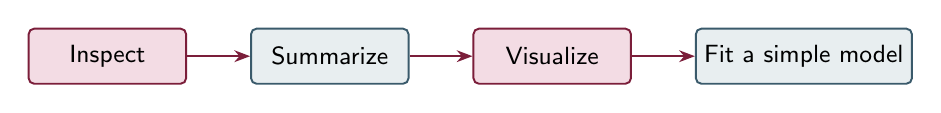
\begin{tikzpicture}[node distance=6mm and 8mm]
        \node[cycstep]                  (ins) {Inspect};
        \node[cycdo, right=of ins]      (sum) {Summarize};
        \node[cycstep, right=of sum]    (vis) {Visualize};
        \node[cycdo, right=of vis]      (fit) {Fit a simple model};
        \draw[flow] (ins) -- (sum);
        \draw[flow] (sum) -- (vis);
        \draw[flow] (vis) -- (fit);
    \end{tikzpicture}
    \end{center}

    \vspace{3mm}
    \begin{block}{What each step means}
        \small
        \emph{Inspect}: what columns and rows does the dataset have, and
        are any values missing? \quad
        \emph{Summarize}: mean, spread, outliers. \quad
        \emph{Visualize}: does the summary match what a plot shows?
        \quad \emph{Fit}: can one quantity predict another?
    \end{block}

    \vspace{2mm}
    \begin{alertblock}{Machine learning is an optional preview}
        The closing section on ML classifiers previews where this path
        leads in later courses. It is \alert{not required} to complete
        the core path above.
    \end{alertblock}
\end{frame}

%===============================================================================
\section{Understanding Engineering Measurements}
%===============================================================================

\begin{frame}{Population vs.\ Sample}
    \leavevmode
    A \alert{population} is every possible measurement that could be
    made. A \alert{sample} is the subset you actually recorded.

    \vspace{2mm}
    \begin{block}{Example}
        A factory produces a million resistors; you measure fifty.
        The million is the population, the fifty are your sample.
        Almost all engineering statistics works from samples --- measuring
        the whole population is usually impossible.
    \end{block}

    \vspace{2mm}
    \textbf{Why it matters computationally:} the \emph{sample} variance
    divides by $N-1$ rather than $N$, to compensate for a small sample
    underestimating the true spread.
\end{frame}

\begin{frame}[fragile]{Population vs.\ Sample Variance in NumPy}
    \leavevmode
\begin{lstlisting}
import numpy as np

readings = np.array([98.2, 101.5, 99.7, 100.3,
                      102.1, 99.1, 100.8])  # ohms

print("Population variance:", np.var(readings))
print("Sample variance:    ", np.var(readings, ddof=1))
\end{lstlisting}
    \texttt{Population variance: 1.588} \\
    \texttt{Sample variance:     1.853}

    \vspace{2mm}
    {\small NumPy computes the population form by default
    (\texttt{ddof=0}) and the sample form when told to
    (\texttt{ddof=1}).}
\end{frame}

\begin{frame}{Mean, Range, Variance, Standard Deviation}
    \leavevmode
    \small
    Four quantities describe most measurement sets adequately.

    \vspace{2mm}
    \begin{columns}[t]
        \begin{column}{.5\textwidth}
            \begin{block}{Mean}
                \scriptsize $\bar{x} = \dfrac{1}{N}\sum_{i=1}^{N} x_i$
                --- the best single estimate of the true value.
            \end{block}
            \vspace{1mm}
            \begin{block}{Range}
                \scriptsize Largest value minus smallest --- crude, but
                instantly informative about outliers.
            \end{block}
        \end{column}
        \begin{column}{.5\textwidth}
            \begin{block}{Variance}
                \scriptsize $\sigma^2 = \dfrac{1}{N}\sum_{i=1}^{N}(x_i -
                \mu)^2$ --- average squared distance from the mean.
            \end{block}
            \vspace{1mm}
            \begin{block}{Standard deviation}
                \scriptsize $\sigma = \sqrt{\sigma^2}$ --- more useful in
                practice since it shares the \alert{same units} as the
                measurement.
            \end{block}
        \end{column}
    \end{columns}
\end{frame}

\begin{frame}[fragile]{Worked Example: Seven Resistors}
    \leavevmode
\begin{lstlisting}
readings = np.array([98.2, 101.5, 99.7, 100.3,
                      102.1, 99.1, 100.8])  # ohms

print(f"Mean:   {np.mean(readings):.2f} ohms")
print(f"Range:  {np.ptp(readings):.2f} ohms")
print(f"Std:    {np.std(readings, ddof=1):.2f} ohms")
\end{lstlisting}
    \texttt{Mean:   100.24 ohms} \quad
    \texttt{Range:  3.90 ohms} \quad
    \texttt{Std:    1.36 ohms}

    \vspace{2mm}
    \begin{block}{Interpret}
        \small Seven $100\,\Omega$ (5\% tolerance) resistors must fall in
        $95$--$105\,\Omega$. Every reading here does --- this batch
        passes.
    \end{block}
\end{frame}

\begin{frame}{Measurement Error: Absolute vs.\ Relative}
    \leavevmode
    When the true value is known independently (a calibrated reference,
    say), measurement quality can be quantified directly.
    \[
    e = x_{\text{measured}} - x_{\text{true}}, \qquad
    \%\,\text{error} = \frac{|e|}{x_{\text{true}}} \times 100 .
    \]

    \vspace{2mm}
    \begin{alertblock}{Why relative error matters}
        An absolute error of $0.243\,\Omega$ is excellent on a
        $100\,\Omega$ resistor, but \alert{catastrophic} on a
        $1\,\Omega$ shunt, where it is a $24\%$ error. The relative form
        lets instruments of different ranges be compared fairly.
    \end{alertblock}
\end{frame}

\begin{frame}{Back to the Bench Dataset}
    \leavevmode
    Summarizing the running bench dataset statistically reveals its
    corrupted reading immediately.

    \vspace{2mm}
    \texttt{temp.mean()} = \texttt{28.28 C} \quad
    \texttt{temp.median()} = \texttt{27.71 C} \quad
    \texttt{temp.max()} = \texttt{98.40 C} \quad
    \texttt{temp.std()} = \texttt{7.06 C}

    \vspace{3mm}
    \begin{block}{Interpret}
        \small Mean and median are close, but the max is wildly out of
        keeping with a board that sits near room temperature. This is
        the signature of a single corrupted sample: the
        \alert{median barely moves}, while the mean and standard
        deviation are inflated. A mean far from the median is often the
        first clue of an outlier --- the IQR rule (later this chapter)
        identifies it precisely.
    \end{block}
\end{frame}

%===============================================================================
\section{Basic Statistical Analysis}
%===============================================================================

\begin{frame}{NumPy/SciPy Statistical Functions}
    \leavevmode
    \small
    \begin{table}
    \striped
    \begin{tabular}{ll}
        \toprule
        \textbf{Function} & \textbf{Description} \\
        \midrule
        \texttt{np.max()} / \texttt{np.min()} & Maximum / smallest value \\
        \texttt{np.mean()} & Average value \\
        \texttt{np.median()} & Median value \\
        \texttt{stats.mode()} & Most frequent value (\texttt{scipy.stats}) \\
        \texttt{np.std()} / \texttt{np.var()} & Standard deviation / variance \\
        \bottomrule
    \end{tabular}
    \end{table}
\end{frame}

\begin{frame}[fragile]{Choosing an Axis: Rows vs.\ Columns}
    \leavevmode
    When performing statistics on a matrix, the \texttt{axis} parameter
    decides the direction.

\begin{lstlisting}
x = np.array([[1, 3], [2, 5], [6, 4]])

print(np.mean(x, axis=0))  # down columns: [3. 4.]
print(np.mean(x, axis=1))  # across rows: [2. 3.5 5.]
print(np.mean(x))          # every element: 3.5
\end{lstlisting}

    \begin{block}{Rule of thumb}
        \texttt{axis=0} collapses \alert{rows} (one result per column).
        \texttt{axis=1} collapses \alert{columns} (one result per row).
        No \texttt{axis} $\to$ one scalar over the whole array.
    \end{block}
\end{frame}

\begin{frame}{Worked Example: Temperature Across Three Cities}
    \leavevmode
    \small
    A user-defined \texttt{datastat()} function computes mean, variance,
    median, max, and min \alert{column-wise} (\texttt{axis=0}) for three
    cities' temperature readings, then optionally plots them.

    \vspace{2mm}
    \texttt{Dataset 1: avg 11.97\ \ \ Dataset 2: avg 8.23\ \ \ Dataset 3: avg 19.87}

    \vspace{3mm}
    \begin{block}{The pattern, not the code}
        Writing a small reusable statistics function once, rather than
        repeating \texttt{np.mean()}/\texttt{np.var()} calls inline,
        is what makes this scale to many datasets.
    \end{block}
\end{frame}

%===============================================================================
\section{Introduction to Data Analytics}
%===============================================================================

\begin{frame}{What Is Data Analytics?}
    \leavevmode
    \alert{Data analytics} examines, cleans, transforms, and interprets
    data to extract insights and inform decisions. Raw data, by itself,
    usually means nothing.

    \vspace{3mm}
    \begin{columns}[t]
        \begin{column}{.5\textwidth}
            \begin{block}{Benefits}
                \scriptsize Informed decisions, efficiency, competitive
                advantage, risk management, cost reduction, predictive
                maintenance.
            \end{block}
        \end{column}
        \begin{column}{.5\textwidth}
            \begin{block}{Domains}
                \scriptsize Business intelligence, healthcare, finance,
                manufacturing, education, energy, public policy.
            \end{block}
        \end{column}
    \end{columns}
\end{frame}

\begin{frame}{The Data Analytics Process}
    \leavevmode
    The first step is always to \alert{define the problem}:
    \begin{itemize}
        \item Why are we losing customers?
        \item Which factors hurt the customer experience?
        \item How can we boost retention while cutting costs?
    \end{itemize}

    \vspace{3mm}
    \begin{block}{Then: find the data}
        Once the problem is defined, determine the best data sources ---
        sensors, databases, surveys, logs --- to help solve it.
    \end{block}
\end{frame}

\begin{frame}{Types of Data}
    \leavevmode
    \small
    \begin{columns}[t]
        \begin{column}{.33\textwidth}
            \begin{block}{Structured}
                \scriptsize Predefined format, rows and columns.
                \emph{E.g.} dates, transaction records.
            \end{block}
        \end{column}
        \begin{column}{.33\textwidth}
            \begin{block}{Unstructured}
                \scriptsize No predefined format. \emph{E.g.} documents,
                images, audio.
            \end{block}
        \end{column}
        \begin{column}{.33\textwidth}
            \begin{block}{Semi-structured}
                \scriptsize Some structure, no rigid schema.
                \emph{E.g.} JSON, server logs.
            \end{block}
        \end{column}
    \end{columns}

    \vspace{3mm}
    {\small Most engineering measurement data in this course is
    \alert{structured} --- the kind pandas handles directly.}
\end{frame}

%===============================================================================
\section{pandas for Data Analytics}
%===============================================================================

\begin{frame}{Why pandas?}
    \leavevmode
    \alert{pandas} is the standard tool for loading, exploring, cleaning,
    and analyzing structured (tabular) data in Python.

    \vspace{2mm}
    \begin{columns}[t]
        \begin{column}{.5\textwidth}
            \begin{block}{Core features}
                \scriptsize Load from CSV/Excel/SQL; explore with
                \texttt{.head()}, \texttt{.shape}, \texttt{.info()};
                summarize with \texttt{.describe()}; filter rows/columns.
            \end{block}
        \end{column}
        \begin{column}{.5\textwidth}
            \begin{block}{Further features}
                \scriptsize Missing data (\texttt{.isnull()},
                \texttt{.fillna()}); grouping (\texttt{.groupby()});
                merging (\texttt{.merge()}, \texttt{.concat()}).
            \end{block}
        \end{column}
    \end{columns}
\end{frame}

\begin{frame}[fragile]{First Look at a Dataset}
    \leavevmode
\begin{lstlisting}
import pandas as pd

df = pd.read_csv('employees.csv')
print(df.head())    # first 5 rows
print(df.shape)     # (1000, 8)
print(df.describe())  # count, mean, std, min, 25/50/75%, max
\end{lstlisting}

    \begin{block}{The routine first pass}
        \small \texttt{.head()}, \texttt{.shape}, and \texttt{.describe()}
        together answer: what does this dataset look like, how big is
        it, and what do the numeric columns typically contain?
    \end{block}
\end{frame}

\begin{frame}{What Is a DataFrame?}
    \leavevmode
    A pandas \alert{DataFrame} is a 2-D, labeled table: rows and columns,
    each column its own data type, built from dictionaries, arrays,
    CSV/Excel files, or SQL.

    \vspace{2mm}
    \begin{block}{Why dictionaries matter here}
        A DataFrame is most easily built from a dictionary --- each key
        becomes a column name, each value the data beneath it. This is
        exactly why the dictionaries from Chapter~3 are worth knowing.
    \end{block}
\end{frame}

\begin{frame}[fragile]{Building a DataFrame}
    \leavevmode
\begin{lstlisting}
Sensor = ['TMP-01', 'TMP-02', 'TMP-03', 'TMP-04']
Readings = [10, 12, 16, 23]

df = pd.DataFrame({'Sensor': Sensor, 'Readings': Readings})
print(df)
print("Mean:", df['Readings'].mean())
\end{lstlisting}
    \texttt{Mean of Readings: 16.0}

    \vspace{2mm}
    {\small Column access (\texttt{df['Readings']}) behaves like a
    labeled NumPy array --- all the usual statistics methods apply.}
\end{frame}

%===============================================================================
\section{Grouping, Cleaning and Outliers}
%===============================================================================

\begin{frame}[fragile]{Data Aggregation with \texttt{groupby}}
    \leavevmode
    Summarizing \emph{by category} --- average power per component type,
    say --- is one of the most common tasks on a loaded dataset.

\begin{lstlisting}
data = {'component':   ['Resistor','Resistor','Capacitor',
                         'Capacitor','Inductor','Inductor'],
        'power_watts': [2.1, 2.4, 1.5, 1.8, 3.2, 3.6]}
df = pd.DataFrame(data)

summary = df.groupby('component')['power_watts'].agg(['mean','sum'])
print(summary)
\end{lstlisting}
    \texttt{Capacitor 1.65 / 3.3\quad Inductor 3.40 / 6.8\quad Resistor 2.25 / 4.5}
\end{frame}

\begin{frame}{Data Cleaning and Preprocessing}
    \leavevmode
    Raw data often contains errors, missing values, and noise. Cleaning
    transforms it into something usable:

    \vspace{2mm}
    \begin{columns}[t]
        \begin{column}{.33\textwidth}
            \begin{block}{Reduction}
                \scriptsize Remove irrelevant data.
            \end{block}
        \end{column}
        \begin{column}{.33\textwidth}
            \begin{block}{Transformation}
                \scriptsize Scale data for modeling compatibility.
            \end{block}
        \end{column}
        \begin{column}{.33\textwidth}
            \begin{block}{Integration}
                \scriptsize Combine multiple sources into one dataset.
            \end{block}
        \end{column}
    \end{columns}

    \vspace{3mm}
    {\small The process begins with \alert{inspection}: find missing
    values, outliers, and inconsistencies.}
\end{frame}

\begin{frame}[fragile]{Finding Missing Values}
    \leavevmode
\begin{lstlisting}
data = {'Node': ['ADC-01','ADC-02','ADC-03',None,'ADC-06'],
        'Samples': [10, None, 16, 18, 20],
        'Voltage': [2.5, 3.0, None, 3.2, 2.9]}
df = pd.DataFrame(data)

missing = df.isnull()
print(df.isnull().sum())   # count per column
\end{lstlisting}
    \texttt{Node: 1\quad Samples: 1\quad Voltage: 1}

    \vspace{2mm}
    {\small \texttt{.isnull()} returns a same-shaped DataFrame of
    \texttt{True}/\texttt{False}; missing values appear as \texttt{NaN}
    (numeric), \texttt{NaT} (datetime), or \texttt{None} (object).}
\end{frame}

\begin{frame}{Detecting Unusual Measurements}
    \leavevmode
    \small
    An outlier is a reading that differs significantly from the rest ---
    it can distort statistics, skew models, or signal a genuine rare
    event.

    \vspace{2mm}
    \begin{alertblock}{A caution worth repeating}
        These methods detect \alert{unusual} observations; they do not
        prove an observation is \alert{wrong}. A statistical test cannot
        tell a sensor fault from a rare but real event --- it can only
        point out where to look.
    \end{alertblock}

    \vspace{2mm}
    Two common methods: the \textbf{Z-score} method ($|Z| > 3$) and the
    \textbf{IQR (Tukey) method}, covered next.
\end{frame}

\begin{frame}{Quartiles and the IQR}
    \leavevmode
    \begin{columns}[t]
        \begin{column}{.5\textwidth}
            \begin{block}{Quartiles}
                \small $Q_1$ (25\%), $Q_2$ (median, 50\%), $Q_3$ (75\%)
                --- quarters of the sorted data.
            \end{block}
            \vspace{2mm}
            \[
            \text{IQR} = Q_3 - Q_1
            \]
        \end{column}
        \begin{column}{.5\textwidth}
            \begin{block}{Tukey's fences ($1.5\times$IQR rule)}
                \small
                \[
                \text{lower} = Q_1 - 1.5\,\text{IQR}
                \]
                \[
                \text{upper} = Q_3 + 1.5\,\text{IQR}
                \]
            \end{block}
        \end{column}
    \end{columns}

    \vspace{3mm}
    {\small Values outside $[\text{lower}, \text{upper}]$ are flagged.
    The multiplier $1.5$ can be adjusted for more or less sensitivity.}
\end{frame}

\begin{frame}{Worked Example: Computing the Bounds}
    \leavevmode
    Data: \texttt{[2, 10, 12, 18, 20, 23, 100]} (sorted).
    \[
    Q_1 = 11, \qquad Q_3 = 21.5, \qquad \text{IQR} = 10.5
    \]
    \[
    \text{lower} = 11 - 1.5(10.5) = -4.75, \qquad
    \text{upper} = 21.5 + 1.5(10.5) = 37.25
    \]

    \vspace{3mm}
    \begin{block}{Result}
        No value is below $-4.75$. The value $100$ exceeds $37.25$ ---
        flagged as an outlier.
    \end{block}
\end{frame}

\begin{frame}[fragile]{Flagging and Handling Outliers}
    \leavevmode
\begin{lstlisting}
Q1 = df['Samples'].quantile(0.25)
Q3 = df['Samples'].quantile(0.75)
IQR = Q3 - Q1
lower, upper = Q1 - 1.5*IQR, Q3 + 1.5*IQR

df['Outlier'] = (df['Samples'] < lower) | (df['Samples'] > upper)
df.loc[df['Outlier'], 'Samples'] = np.nan   # or: replace with median
\end{lstlisting}

    \begin{block}{Two common fixes once flagged}
        \small Replace with \texttt{NaN} (then treat as missing data), or
        replace with the column \alert{median} --- a single outlier
        barely moves the median, making it a safe stand-in.
    \end{block}
\end{frame}

\begin{frame}{A Boxplot Shows the Same Test Graphically}
    \leavevmode
    \begin{columns}[t]
        \begin{column}{.5\textwidth}
            \begin{itemize}
                \item Box spans $Q_1$ to $Q_3$ (middle 50\%).
                \item Line inside the box is the median.
                \item Whiskers extend to the Tukey bounds.
                \item Points beyond the whiskers are outliers.
            \end{itemize}
        \end{column}
        \begin{column}{.5\textwidth}
            \small
            \texttt{plt.boxplot(samples, vert=False)} draws exactly this
            --- a visual cross-check on the numeric IQR calculation.
        \end{column}
    \end{columns}

    \vspace{3mm}
    {\small Missing data and outliers are the two issues that most
    commonly compromise an analysis --- both require deliberate,
    documented handling.}
\end{frame}

%===============================================================================
\section{Data Analysis and Visualization}
%===============================================================================

\begin{frame}{Three Levels of Data Analysis}
    \leavevmode
    \begin{table}
    \striped
    \small
    \begin{tabular}{p{2.1cm}p{3cm}p{5.5cm}}
        \toprule
        \textbf{Type} & \textbf{Key Question} & \textbf{Focus} \\
        \midrule
        Descriptive & What happened? & Summarize historical data, find patterns \\
        Predictive & What could happen? & Forecast from historical patterns \\
        Prescriptive & What's the best action? & Choose the best course of action \\
        \bottomrule
    \end{tabular}
    \end{table}
\end{frame}

\begin{frame}[fragile]{Descriptive Analytics: One and Two Variables}
    \leavevmode
    \small
    \textbf{Univariate} describes a single variable (mean, median, mode).
    \textbf{Bivariate} examines the relationship between two.

\begin{lstlisting}
heights = [157, 163, 176, 152]
print("Mean:", np.mean(heights))     # univariate

plt.scatter(temperature, sales)      # bivariate: relationship
\end{lstlisting}

    {\small Together, these summarize large datasets, reveal patterns,
    and flag issues \emph{before} any modeling is attempted.}
\end{frame}

\begin{frame}[fragile]{Predictive Analytics: A First Regression}
    \leavevmode
\begin{lstlisting}
from sklearn.linear_model import LinearRegression

X = [[26], [30], [35], [40]]   # temperature
y = [1000, 2500, 3500, 4500]   # sales

model = LinearRegression()
model.fit(X, y)
print(model.predict([[32]]))   # Predicted sales: [2693.0]
\end{lstlisting}

    \begin{block}{What just happened}
        \small The model learned the best-fit straight line relating
        temperature to sales --- a typical example of
        \alert{supervised learning} with a single feature.
    \end{block}
\end{frame}

\begin{frame}{Prescriptive Analytics and Visualizing an Analysis}
    \leavevmode
    \small
    \textbf{Prescriptive analytics} recommends actions, not just
    predictions --- \texttt{if predicted\_sales > 5000: increase
    production}.

    \vspace{3mm}
    \begin{block}{Visualizing the dataset, not the signal}
        Once data is loaded, cleaned, and aggregated, a chart is usually
        the fastest way to communicate what was found. A \alert{bar
        chart} compares categories (e.g.\ a \texttt{groupby} summary); a
        \alert{scatter plot} shows a relationship between two variables.
    \end{block}
\end{frame}

%===============================================================================
\section{Machine Learning (Optional Preview)}
%===============================================================================

\begin{frame}{Machine Learning: An Optional Preview}
    \leavevmode
    \begin{alertblock}{Before you continue}
        This section previews where the core path leads in later
        courses. It is \alert{not required} to understand the rest of
        this course --- treat it as a survey, not a deep dive.
    \end{alertblock}

    \vspace{3mm}
    Predictive analytics uses machine learning: models learn from
    historical data and are used for prediction and classification,
    without being explicitly programmed for the specific task.
\end{frame}

\begin{frame}{Regression vs.\ Classification}
    \leavevmode
    Predictive models divide into two kinds, by what they produce:

    \vspace{2mm}
    \begin{columns}[t]
        \begin{column}{.5\textwidth}
            \begin{block}{Regression}
                \small Predicts a \alert{quantity} --- a temperature, a
                voltage, a time constant. \\
                \emph{``How hot will this motor get?''}
            \end{block}
        \end{column}
        \begin{column}{.5\textwidth}
            \begin{block}{Classification}
                \small Predicts a \alert{category} --- healthy or
                faulty, pass or fail. \\
                \emph{``Is this motor overheating?''}
            \end{block}
        \end{column}
    \end{columns}
\end{frame}

\begin{frame}[fragile]{A Simple Decision Tree}
    \leavevmode
\begin{lstlisting}
from sklearn.tree import DecisionTreeClassifier

X = [[1], [2], [3], [4]]
y = ['low', 'low', 'high', 'high']

model = DecisionTreeClassifier()
model.fit(X, y)
print(model.predict([[3]]))   # 'high'
\end{lstlisting}

    \begin{alertblock}{A model has no sense of its own limits}
        Asked to classify $99$ --- far outside its training data --- it
        still returns \texttt{high} regardless, since its only rule is
        ``above 2.5''. Judging when a question falls outside the
        model's experience remains the engineer's job.
    \end{alertblock}
\end{frame}

\begin{frame}{The General Machine Learning Workflow}
    \leavevmode
    \begin{center}
    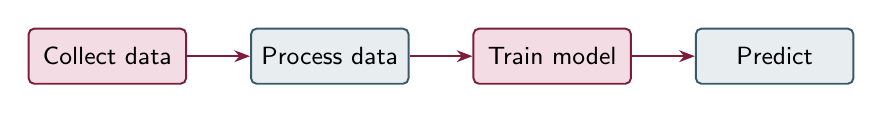
\begin{tikzpicture}[node distance=6mm and 8mm]
        \node[cycstep]                  (c) {Collect data};
        \node[cycdo, right=of c]        (p) {Process data};
        \node[cycstep, right=of p]      (t) {Train model};
        \node[cycdo, right=of t]        (u) {Predict};
        \draw[flow] (c) -- (p);
        \draw[flow] (p) -- (t);
        \draw[flow] (t) -- (u);
    \end{tikzpicture}
    \end{center}

    \vspace{3mm}
    \begin{block}{Why training and testing sets are split}
        A model evaluated only on the data it \alert{memorized} tells
        you nothing about how it performs on new measurements --- always
        hold out a test set.
    \end{block}
\end{frame}

\begin{frame}{Three Types of Machine Learning}
    \leavevmode
    \small
    \begin{columns}[t]
        \begin{column}{.33\textwidth}
            \begin{block}{Supervised}
                \scriptsize Learns from \alert{labeled} training data.
                \emph{E.g.} regression, classification.
            \end{block}
        \end{column}
        \begin{column}{.33\textwidth}
            \begin{block}{Unsupervised}
                \scriptsize Learns from \alert{unlabeled} data, finding
                patterns on its own.
            \end{block}
        \end{column}
        \begin{column}{.33\textwidth}
            \begin{block}{Reinforcement}
                \scriptsize Learns through \alert{feedback}, reinforcing
                correct responses.
            \end{block}
        \end{column}
    \end{columns}

    \vspace{3mm}
    {\small This course's examples are all \alert{supervised} ---
    regression and decision-tree classification.}
\end{frame}

\begin{frame}{Where This Leaves You}
    \leavevmode
    \small
    \begin{itemize}
        \item The \alert{core path} --- inspect, summarize, visualize,
              fit a simple model --- is what every engineering dataset
              needs, regardless of whether machine learning is involved.
        \item \texttt{LinearRegression} and
              \texttt{DecisionTreeClassifier} are two simple, inspectable
              starting points, not the final word.
        \item Neither can be trusted outside the range of data it was
              trained on: machine learning is \alert{one more
              engineering tool}, not a substitute for understanding the
              problem.
    \end{itemize}

    \vspace{4mm}
    \begin{center}
        \large\color{primary}\textbf{This concludes the taught chapters
        of the course.}
    \end{center}
\end{frame}

\end{document}
